% concatenated from cvector_projection_paper.tex
\documentclass[11pt, a4paper]{amsart}

\usepackage{amsmath, amssymb, amsthm}
\usepackage{mathtools}
\usepackage{enumitem}
\usepackage{hyperref}
\usepackage{tikz}
\usepackage{booktabs}

\hypersetup{
  colorlinks=true,
  linkcolor=blue!60!black,
  citecolor=green!50!black,
  urlcolor=blue!70!black
}

\newtheorem{theorem}{Theorem}[section]
\newtheorem{proposition}[theorem]{Proposition}
\newtheorem{lemma}[theorem]{Lemma}
\newtheorem{corollary}[theorem]{Corollary}
\theoremstyle{definition}
\newtheorem{definition}[theorem]{Definition}
\newtheorem{example}[theorem]{Example}
\newtheorem{remark}[theorem]{Remark}

\newcommand{\ZZ}{\mathbb{Z}}
\newcommand{\QQ}{\mathbb{Q}}
\newcommand{\RR}{\mathbb{R}}
\newcommand{\cA}{\mathcal{A}}
\newcommand{\cC}{\mathcal{C}}
\DeclareMathOperator{\indeg}{indeg}

\title[Banded projections of affine $c$-vectors]{%
  Banded coordinate projections of $c$-vectors in affine type}

\author{Sarah B.\ Brodsky}

\subjclass[2020]{Primary 13F60; Secondary 05E10, 16G20}
\keywords{cluster algebras, $c$-vectors, affine type, real Schur roots,
tubes, annulus}

\date{\today}

\begin{document}

\begin{abstract}
For an acyclic cluster algebra, the $c$-vectors are, up to sign, the real
Schur roots of the associated root system. We study the two-coordinate
projections $(c_v, c_w)$ of this configuration: when the difference
$c_v - c_w$ is bounded, the image lies in a finite band of lattice lines,
and we ask when the projection fills every lattice point of that band. In
affine type, boundedness is equivalent to $\delta_v=\delta_w$ for the null
root $\delta$. Writing this common coordinate as $r$, we prove that a band
line fills exactly when its transjective root classes cover every residue
modulo $r$. This yields a complete classification for every acyclic
orientation of every simply-laced affine diagram. For a source-sink
$\widetilde A_n$ quiver, every projection fills except the source-sink
diagonal. In tree type, every width-one band fills, while every width-two
band fails on its two boundary lines because of a congruence gap. The
Auslander--Reiten defect further determines whether such a boundary line is
finite or contains an infinite arithmetic progression; finiteness is
governed by a balanced-geodesic criterion. On the annulus, the absolute
defect is the crossing number with the core curve, and the $\delta$-shift is
the Dehn twist along it.
\end{abstract}

\maketitle

\section{Introduction}
\label{sec:intro}

Let $Q$ be an acyclic quiver on vertex set $Q_0$, and let $\cA(Q)$ be the
cluster algebra with principal coefficients at the seed associated with
$Q$. The $c$-vectors of $\cA(Q)$, collected over all seeds, form a finite
or infinite subset $C(Q) \subset \ZZ^{Q_0}$; by sign-coherence
\cite{GHKK2018} each $c$-vector is either nonnegative or nonpositive, and
by N\'ajera Ch\'avez \cite{NajeraChavez2013} the positive $c$-vectors are
exactly the real Schur roots of $Q$, the dimension vectors of the
exceptional indecomposable representations. Thus
\[
  C(Q) \;=\; \{\, \pm\beta : \beta \text{ a real Schur root of } Q \,\}.
\]

For a pair of vertices $v, w \in Q_0$ we consider the coordinate
projection
\[
  \pi_{vw} \colon \ZZ^{Q_0} \to \ZZ^2,
  \qquad
  \pi_{vw}(c) = (c_v, c_w).
\]
When the difference $c_v - c_w$ is bounded over $C(Q)$, the image
$\pi_{vw}(C(Q))$ is contained in a finite union of lattice lines, the
\emph{band} $\{(x, y) : |x - y| \leq b_{vw}\}$ with $b_{vw} = \sup_{c}|c_v
- c_w|$. In finite and affine type, the present paper answers two questions: for
which pairs is the difference bounded, and, when it is, when does
$\pi_{vw}$ surject onto the band.

Two things make these questions natural. First, the $c$-vector set is a
fundamental mutation-theoretic object: it records the tropical dynamics of the
coefficients \cite{FominZelevinsky2007, NakanishiZelevinsky2012}, it is
sign-coherent \cite{GHKK2018}, and in the acyclic case it is the set of
signed real Schur roots \cite{NajeraChavez2013, SpeyerThomas2013}, so
questions about its geometry are questions about the root system seen
through the cluster structure. Coordinate projections are the simplest
two-dimensional shadows of this configuration; the band is exactly the
region a bounded-difference shadow can occupy, and filling is the
completeness question for the shadow. Second, the answer is not merely
combinatorial: the Auslander--Reiten defect determines which affine root
classes generate infinite progressions, while the null-root coordinates
determine the congruence classes of those progressions. Together they give
a complete failure classification over every simply-laced affine type and
every acyclic orientation (Section~\ref{sec:classification}). In the annulus the story has a
topological reading, in the line of the descriptions of $c$-vectors by
curves on surfaces \cite{FominShapiroThurston2008, Hong2021,
LeeLeeMills2019}: the positive $c$-vectors are represented by arcs, the
absolute defect is the crossing number with the core curve, and the
$\delta$-shift is the Dehn twist along it (Section~\ref{sec:surface}).

The first question has a uniform answer in finite and affine type; in the
affine case it is governed by the null root.

\begin{theorem}[Band-existence dichotomy]
\label{thm:band_dichotomy}
Let $Q$ be an acyclic quiver. If $Q$ is of finite type, then $C(Q)$ is
finite, so every coordinate difference is bounded. If $Q$ is of affine
type with null root $\delta$, then for $v, w \in Q_0$,
\[
  \sup_{c \in C(Q)} |c_v - c_w| < \infty
  \qquad\Longleftrightarrow\qquad
  \delta_v = \delta_w,
\]
and when $\delta_v = \delta_w$ one has
$b_{vw} = \max_{\alpha} |\alpha_v - \alpha_w|$ over the real roots
$\alpha$ of the underlying finite root system.
\end{theorem}

In type $\widetilde{A}_n$ the null root is $\delta = (1, \dots, 1)$, so
\emph{every} pair is banded, with $b_{vw} = 1$. These are the cluster
algebras of the annulus \cite{FominShapiroThurston2008}. We work throughout
with the \emph{source-sink orientation} of the $(n+1)$-cycle: an acyclic
orientation with a \emph{unique} source $s$ and a \emph{unique} sink $t$,
which divide the cycle into two oriented paths $s \to t$ of lengths $p$ and
$q$ with $p + q = n + 1$. \textup{(}Not every acyclic orientation of the
cycle is of this form: the alternating orientation has several sources and
sinks, and a different filling pattern; we return to this seed-dependence in
Remark~\ref{rem:seed_dependence}.\textup{)} In the surface model the two
oriented paths correspond to the two boundary components, carrying $p$ and
$q$ marked points, and the two non-homogeneous tubes have ranks $p$ and $q$.
Our main result resolves the surjectivity question completely for this seed.

\begin{theorem}[Projection-filling]
\label{thm:main}
Let $Q$ be a source-sink orientation of the $(n+1)$-cycle, with unique source
$s$ and unique sink $t$. Then:
\begin{enumerate}[label=\textup{(\arabic*)}]
\item every coordinate difference satisfies $|c_v - c_w| \leq 1$, so the
  band is $\{|c_v - c_w| \leq 1\}$;
\item for every pair $(v, w)$ other than $(s, t)$, the projection
  $\pi_{vw}$ surjects onto the full band;
\item for the source-sink pair, $\pi_{st}(C(Q))$ is the band with the
  diagonal $\{c_s = c_t\}$ removed except for a bounded segment; the
  diagonal carries only the regular part of $C(Q)$.
\end{enumerate}
In particular the source-sink diagonal $\{c_s = c_t\}$ is the unique
non-filled band line.
\end{theorem}

The mechanism is transparent once the right invariant is identified. The
defect form of the tame hereditary algebra $kQ$, which separates
preprojective, regular, and preinjective modules, turns out to be the
\emph{coordinate difference of source and sink},
\[
  \partial(x) \;=\; x_s - x_t,
\]
a one-line consequence of the source having in-degree $0$ and the sink
in-degree $2$ in the cycle (Lemma~\ref{lem:defect}). Consequently an arc
is transjective exactly when it contains exactly one of $\{s, t\}$, and
the source-sink diagonal $\{c_s = c_t\}$ is exactly the defect-zero
locus, where only the finitely many regular real Schur roots live. Every
other line is reached by a transjective root, whose $\delta$-shifts sweep
the entire line; the realizers are supplied by two short constructions
(Section~\ref{sec:main}).

This gives the result a meaning beyond the combinatorics
(Section~\ref{sec:defect_meaning}). The defect is the canonical bounded
invariant whose zero-level is the finite set of exceptional regular roots
(Proposition~\ref{prop:defect_obstruction}). On the \emph{diagonal}, the
complete classification shows that non-filling occurs only when the defect
is the coordinate difference $x_v-x_w$: this is the source-sink pair of
$\widetilde A_n$ in its source-sink orientation
(Theorem~\ref{thm:complete_classification}). There
the three band lines
of $\pi_{st}$ are the preprojective, regular, and preinjective strata
(Theorem~\ref{thm:defect_detection}).

Off the diagonal a second mechanism appears. If
$r=\delta_v=\delta_w$, a $\delta$-shift advances the projection by
$(r,r)$, so one transjective root class covers only one residue modulo $r$.
The residue criterion of Lemma~\ref{lem:filling_criterion} turns this into
a complete classification. Every banded pair of coefficient one fills,
apart from the source-sink diagonal. In tree type every width-one band
fills, while the boundary lines of every width-two band fail. These are the
nonadjacent spine pairs of $\widetilde D_n$, the pair $(3,6)$ of
$\widetilde E_7$, and the pairs $(1,6)$, $(2,5)$, $(3,7)$ of
$\widetilde E_8$; types $\widetilde D_4$, $\widetilde D_5$, and
$\widetilde E_6$ fill completely. The defect then refines, rather than
causes, this congruence failure: a balanced extremal root is regular and
leaves a finite boundary line, whereas a nonzero-defect extremal root
generates an infinite arithmetic progression without filling the other
residues. This is the orientation-dependent balance law of
Theorem~\ref{thm:complete_classification}.

The squarefree Pr\"ufer $4$-cycle on $\{1, 2, 3, 6\}$, an acyclic
orientation of the $4$-cycle of affine type $\widetilde{A}_3$, is the
smallest nontrivial instance; there the source-sink pair is $(1, 6)$,
and Theorem~\ref{thm:main} recovers by hand the projection structure we
work out in Section~\ref{sec:example}.

\medskip\noindent\textbf{Conventions.}\;
All quivers are finite, connected, simply-laced, and without loops or
$2$-cycles. We work over an algebraically closed field $k$, and identify a real root
with the dimension vector of the corresponding exceptional module. For a
subset $I \subseteq Q_0$ we write $\alpha_I = \sum_{i \in I} e_i$ for its
indicator vector.

\section{Preliminaries}
\label{sec:prelim}

In this section, we recall the facts about acyclic cluster algebras and
tame hereditary algebras that we use. We refer to
\cite{FominZelevinsky2007} for cluster algebras with principal
coefficients and $c$-vectors, to \cite{NajeraChavez2013, GHKK2018} for the
identification of $c$-vectors with real Schur roots, and to
\cite{Ringel1984, Kac1990} for the representation theory of tame
hereditary algebras and affine root systems.

\subsection*{\texorpdfstring{$c$-vectors}{c-vectors} and real Schur roots}
The $c$-vectors of $\cA(Q)$ at a seed $t$ are the columns of the $c$-matrix
$C^t$, which tracks the principal coefficients. By sign-coherence
\textup{(}\cite[Corollary~5.5]{GHKK2018}; for the skew-symmetric case,
Derksen--Weyman--Zelevinsky \cite{DWZ2010}\textup{)} each $c$-vector is
nonnegative or nonpositive, and by N\'ajera Ch\'avez
\cite[Theorem~1.3]{NajeraChavez2013} the positive $c$-vectors of an acyclic
cluster algebra are exactly the real Schur roots of $Q$, that is, the
dimension vectors of the exceptional (rigid, indecomposable) $kQ$-modules.
Hence $C(Q)$ is the set of signed real Schur roots. The $c$-vectors of affine
and tame type are thus governed by the tame hereditary representation theory
of $Q$ \cite{Ringel1984}; we use this dictionary throughout. To the best of
our knowledge the coordinate projections of the configuration $C(Q)$, and the
filling question studied here, have not been considered before.

\subsection*{Type classification}
By the Fomin--Zelevinsky classification \cite{FominZelevinsky2003II}, an
acyclic cluster algebra is of finite type if and only if the underlying
graph of $Q$ is a Dynkin diagram, and of affine (tame) type if and only
if that graph is a Euclidean diagram. The acyclic orientations of the
$(n+1)$-cycle are exactly the connected quivers of affine type
$\widetilde{A}_n$.

\subsection*{Roots of affine type}
Since $Q$ is acyclic its Euler form is unitriangular and its symmetrized
Tits form is the affine quadratic form, which is positive semidefinite
with one-dimensional radical $\ZZ\delta$ spanned by the null root
$\delta$. The real roots of a simply-laced affine root system are exactly
\[
  \{\, \alpha + m\delta : \alpha \in \Delta_{\mathrm{fin}},\ m \in \ZZ \,\},
\]
where $\Delta_{\mathrm{fin}}$ is the underlying finite root system
\cite[Ch.~6]{Kac1990}. In type $\widetilde{A}_n$ one has
$\delta = (1, \dots, 1)$, and $\Delta_{\mathrm{fin}} = A_n$; the positive
roots of $A_n$ obtained by deleting a vertex of the cycle are the
indicators of cyclic intervals, so the real roots of $\widetilde{A}_n$
are
\[
  \{\, \pm \alpha_I + m\delta : I \text{ a cyclic interval},\ m \in \ZZ \,\}.
\]

\subsection*{Preprojective, regular, preinjective}
For a tame hereditary algebra the indecomposable modules split into three
families: preprojective, regular, and preinjective. The
\emph{transjective} modules are the preprojective and the preinjective
ones; the regular modules lie in tubes, of which all but finitely many
are homogeneous (rank $1$) and the rest are non-homogeneous. In type
$\widetilde{A}_n$ there are two non-homogeneous tubes, of ranks $p$ and
$q$; in types $\widetilde{D}$ and $\widetilde{E}$ there are three. The
defect $\partial$ is the linear form on the
Grothendieck group with $\partial(M) < 0$, $= 0$, $> 0$ according as $M$
is preprojective, regular, or preinjective; a real root is regular if and
only if its defect vanishes \cite{Ringel1984}. Preprojective and
preinjective modules are directing, hence exceptional, so every
transjective real root is a real Schur root. In a tube of rank $r$ the
exceptional regular modules are exactly those of quasi-length less than
$r$, finitely many.

We will use the following consequence repeatedly. It also fixes the sign
convention for affine shifts: a signed $c$-vector need not itself be a
dimension vector.

\begin{lemma}[Box roots and signed shifts]
\label{lem:box_schur}
Let $Q$ be acyclic of affine type. If $\beta$ is a positive real root with
$0 \leq \beta \leq \delta$ componentwise, then $\beta$ is a real Schur
root. If, in addition, $\partial(\beta) \neq 0$, then
$\beta + m\delta \in C(Q)$ for every $m \in \ZZ$.
\end{lemma}

\begin{proof}
If $\partial(\beta) \neq 0$, then $\beta$ is transjective and hence
exceptional. Suppose that $\partial(\beta) = 0$. The indecomposable of
dimension vector $\beta$ lies in a tube of rank $r$. If its quasi-length
were at least $r$, its regular composition factors would contain a full
period, whose dimension vectors sum to $\delta$. The inequality
$\beta \leq \delta$ would then force $\beta = \delta$, which is impossible
because $\beta$ is real. Thus the quasi-length is less than $r$, so the
indecomposable is exceptional. This proves the first assertion.

Now suppose that $\partial(\beta) \neq 0$. For $m \geq 0$, the root
$\beta + m\delta$ is positive and transjective, hence a positive
$c$-vector. If $m \leq -1$, then
\[
  \beta + m\delta
  = -\bigl((\delta - \beta) + (-m-1)\delta\bigr).
\]
Since $\delta$ lies in the radical of the Tits form,
$q(\delta-\beta)=q(\beta)=1$; thus $\delta - \beta$ is a positive real root.
It has defect $-\partial(\beta) \neq 0$; therefore the vector in parentheses is a
positive transjective $c$-vector. Its negative is a $c$-vector as well, as
desired.
\end{proof}

\section{The band-existence dichotomy}
\label{sec:band}

In this section, we prove Theorem~\ref{thm:band_dichotomy}, valid in
finite and affine type.

\begin{proof}[Proof of Theorem~\ref{thm:band_dichotomy}]
If $Q$ is of finite type, then $C(Q)$ is a finite set of roots, so every
coordinate difference is bounded.

Suppose $Q$ is of affine type. By the preliminaries every $c$-vector is a
real root $\alpha + m\delta$ with $\alpha \in \Delta_{\mathrm{fin}}$ and
$m \in \ZZ$, whence
\[
  c_v - c_w \;=\; \alpha_v - \alpha_w + m\,(\delta_v - \delta_w).
\]
The set $\{\alpha_v - \alpha_w : \alpha \in \Delta_{\mathrm{fin}}\}$ is
finite. If $\delta_v = \delta_w$, the term in $m$ vanishes, so
$|c_v - c_w| \leq \max_\alpha |\alpha_v - \alpha_w| < \infty$. If
$\delta_v \neq \delta_w$, recall that the transjective real roots are
real Schur roots, hence $c$-vectors, and that there are infinitely many of
them, the preprojective and preinjective components each being infinite
\textup{(}\cite[\S3]{Ringel1984}\textup{)}. Each such root is
$\alpha + m\delta$ with $\alpha \in \Delta_{\mathrm{fin}}$, and
$\Delta_{\mathrm{fin}}$ is finite, so $|m|$ is unbounded over them. As
$\delta_v \neq \delta_w$, the difference $c_v - c_w = \alpha_v -
\alpha_w + m(\delta_v - \delta_w)$ has bounded $\alpha$-part and unbounded
$m$-term, hence is unbounded. Finally the displayed bound is sharp: after
replacing a finite root by its negative, write it as a positive finite root
$\alpha$; the representatives $\alpha$ and $\delta-\alpha$ both lie
componentwise between $0$ and $\delta$, and are real Schur roots by
Lemma~\ref{lem:box_schur}. Thus a finite root attaining the displayed
maximum is, up to sign and addition of $\delta$, a $c$-vector with the same
absolute coordinate difference. This proves the equivalence and the stated
value of $b_{vw}$.
\end{proof}

\begin{example}[The dichotomy in type $\widetilde{D}_4$]
\label{ex:D4}
Let $Q$ be the $4$-subspace quiver: a central vertex $0$ and four leaves
$1, 2, 3, 4$, with any acyclic orientation of the four edges. The null
root is $\delta = (2, 1, 1, 1, 1)$, with the central coordinate equal to
$2$. By Theorem~\ref{thm:band_dichotomy}, the six leaf-leaf pairs are
banded, while the four center-leaf pairs are not. A direct enumeration of
$c$-vectors confirms this: the leaf-leaf differences never exceed $1$,
whereas each center-leaf difference takes arbitrarily large values.
\end{example}

\section{The defect form in type \texorpdfstring{$\widetilde{A}_n$}{An}}
\label{sec:defect}

In this section, we identify the defect form of an acyclic cycle quiver
and deduce the transjective criterion. Fix a source-sink orientation $Q$ of
the $(n+1)$-cycle, with unique source $s$ and unique sink $t$.

\begin{lemma}[Defect and transjective criterion]
\label{lem:defect}
For any acyclic orientation of the $(n+1)$-cycle, with sources $s_1, \dots,
s_k$ and sinks $t_1, \dots, t_k$, the defect form of $kQ$ is, up to sign,
\[
  \partial(x) \;=\; \sum_{i=1}^{k} x_{s_i} - \sum_{i=1}^{k} x_{t_i};
\]
this is a coordinate difference if and only if $k = 1$, that is, the source
and sink are unique, in which case $\partial(x) = x_s - x_t$. Under that
\textup{(}standing\textup{)} hypothesis a cyclic interval indicator
$\alpha_I$ is regular if and only
if $I$ contains both or neither of $\{s, t\}$, and transjective if and
only if $I$ contains exactly one of $\{s, t\}$. Moreover, if $\alpha_I$ is
transjective, then $\alpha_I + m\delta$ is a $c$-vector for every
$m \in \ZZ$, whereas the regular part of $C(Q)$ is finite.
\end{lemma}

\begin{proof}
The defect is $\partial(x) = \langle \delta, x \rangle$, where
$\langle x, y \rangle = \sum_{i} x_i y_i - \sum_{i \to j} x_i y_j$ is the
Euler form. Since $\delta = (1, \dots, 1)$,
\[
  \partial(x)
  \;=\; \sum_i x_i - \sum_{i \to j} x_j
  \;=\; \sum_i x_i - \sum_{j} \indeg(j)\, x_j.
\]
In the $(n+1)$-cycle every vertex has degree $2$, so a source has in-degree
$0$, a sink in-degree $2$, and every other vertex in-degree $1$; hence
$\sum_j \indeg(j)\, x_j = \sum_j x_j + \sum_i x_{t_i} - \sum_i x_{s_i}$, and
\[
  \partial(x) \;=\; \sum_i x_i - \Bigl(\sum_j x_j + \sum_i x_{t_i}
  - \sum_i x_{s_i}\Bigr) \;=\; \sum_i x_{s_i} - \sum_i x_{t_i}.
\]
This has $2k$ nonzero coefficients, so it is a coordinate difference exactly
when $k = 1$, giving $\partial(x) = x_s - x_t$; we assume this from now on.
A real root is regular if and only if its defect vanishes
\cite{Ringel1984}; for a $0/1$ indicator $\alpha_I$ this means
$(\alpha_I)_s = (\alpha_I)_t$, that is, $I$ contains both or neither of
$\{s, t\}$. Otherwise $\partial(\alpha_I) = \pm 1$ and $\alpha_I$ is
transjective, which happens exactly when $I$ contains one of $\{s, t\}$.

For the last statement, the defect is unchanged by adding $\delta$, since
$\partial(\delta) = \delta_s - \delta_t = 0$. Thus if $\alpha_I$ is
transjective, Lemma~\ref{lem:box_schur} gives
$\alpha_I + m\delta \in C(Q)$ for every $m \in \ZZ$. The regular real Schur
roots are the exceptional regular modules; each of the two
non-homogeneous tubes contributes finitely many, and the homogeneous
tubes contain no exceptional modules, so the regular part of $C(Q)$ is
finite, as desired.
\end{proof}

\section{The projection-filling theorem}
\label{sec:main}

In this section, we prove Theorem~\ref{thm:main}. We keep $Q$, $s$, $t$
as above, and we say a band line $\{c_v - c_w = d\}$ is \emph{filled} if
$\pi_{vw}(C(Q))$ contains every integer point of it.

We first record the elementary but decisive observation that a single
transjective root fills its whole line.

\begin{lemma}[Transjective roots fill]
\label{lem:fills}
Let $\alpha_I$ be a transjective cyclic interval and set
$d = (\alpha_I)_v - (\alpha_I)_w$. Then the line $\{c_v - c_w = d\}$ is
filled.
\end{lemma}

\begin{proof}
By Lemmas~\ref{lem:defect} and~\ref{lem:box_schur},
$\alpha_I + m\delta \in C(Q)$ for every
$m \in \ZZ$. Its projection is
$\pi_{vw}(\alpha_I + m\delta) = ((\alpha_I)_v + m,\, (\alpha_I)_w + m)$,
which runs over every integer point of $\{c_v - c_w = d\}$ as $m$ varies, as
desired.
\end{proof}

Observe that, by applying the sign $-1$, a transjective root with
difference $d$ also fills the line $\{c_v - c_w = -d\}$. We now produce
transjective realizers for every line except the source-sink diagonal.

\begin{proof}[Proof of Theorem~\ref{thm:main}]
\textbf{(1)}\; By Theorem~\ref{thm:band_dichotomy} with
$\delta = (1, \dots, 1)$, every difference is bounded, and the bound is
$\max_\alpha |\alpha_v - \alpha_w| = 1$ since the finite roots of $A_n$
are signed interval indicators.

\textbf{(2) and the filled lines.}\; Fix a pair $(v, w)$ and a value
$d \in \{-1, 0, 1\}$. By Lemma~\ref{lem:fills} it suffices to exhibit a
transjective cyclic interval $I$ with $(\alpha_I)_v - (\alpha_I)_w = d$,
that is, by Lemma~\ref{lem:defect}, an interval containing exactly one of
$\{s, t\}$ with the prescribed relation to $v, w$.

\emph{The lines $d = \pm 1$.} We treat $d = +1$, where the interval must
contain $v$ and not $w$; the case $d = -1$ is symmetric. If
$v \in \{s, t\}$, the singleton $\{v\}$ contains exactly one of
$\{s, t\}$ and excludes $w \neq v$, as required. If $v \notin \{s, t\}$,
let $I_s$ be the unique arc from $v$ to $s$ avoiding $t$, and $I_t$ the
unique arc from $v$ to $t$ avoiding $s$; each exists because deleting the
avoided vertex opens the cycle into a path containing both endpoints.
Then $I_s$ contains $s$ but not $t$, and $I_t$ contains $t$ but not $s$,
so both are transjective, and both contain $v$. They leave $v$ toward
different neighbors: if they shared a first edge, then walking from $v$
along it we would meet one of $s, t$ before the other, and the arc avoiding
that vertex could not have used the edge. Hence $I_s \cap I_t = \{v\}$.
Since $w \neq v$, at least one of $I_s, I_t$ excludes $w$, and that interval
is the desired realizer.

\emph{The lines $d = 0$.} Here the interval must contain both or neither
of $\{v, w\}$. The singleton $\{s\}$ is transjective, and it contains
neither $v$ nor $w$ precisely when $s \notin \{v, w\}$; likewise $\{t\}$
works precisely when $t \notin \{v, w\}$. If $\{v, w\} \neq \{s, t\}$,
then at least one of $s, t$ lies outside $\{v, w\}$, so the corresponding
singleton fills the line $d = 0$.

Thus for every pair $(v, w) \neq (s, t)$ all three lines $d \in
\{-1, 0, 1\}$ are filled, proving (2); and for the pair $(s, t)$ the
lines $d = \pm 1$ are filled by $\{s\}$ and $\{t\}$.

\textbf{(3) The source-sink diagonal.}\; For the pair $(s, t)$ and
$d = 0$, the condition $(\alpha_I)_s = (\alpha_I)_t$ is the defect-zero
condition, so by Lemma~\ref{lem:defect} no transjective interval realizes
it; only regular roots lie on the diagonal $\{c_s = c_t\}$. The regular
part of $C(Q)$ is finite (Lemma~\ref{lem:defect}), so the diagonal
carries only finitely many $c$-vectors and is not filled. This is the
unique non-filled band line, as desired.
\end{proof}

\begin{remark}[Invariant phrasing]
\label{rem:invariant}
The exceptional locus is intrinsic: it is the defect-zero line of the
source-sink pair,
\[
  \{c_s = c_t\} \;=\; \{\partial = 0\}.
\]
Equivalently, it is the projection direction along which the two tubes,
and only the tubes, are seen. Theorem~\ref{thm:main} thus reads: \emph{the
$c$-vector set of an annulus cluster algebra surjects onto the full
bounded-difference band in every coordinate pair, except along the
defect-zero line of the source-sink pair, where only its regular part
lives.}
\end{remark}

\section{The squarefree Pr\"ufer \texorpdfstring{$4$}{4}-cycle}
\label{sec:example}

In this section, we work out the smallest nontrivial case, the
$\widetilde{A}_3$ cluster algebra of the $4$-cycle, in the orientation
arising from the divisibility order on the squarefree integers with prime
factors in $\{2, 3\}$.

\begin{example}[$\widetilde{A}_{2,2}$]
\label{ex:prufer}
Let $V = \{1, 2, 3, 6\}$, with arrows recording multiplication by a
prime,
\[
  1 \to 2, \qquad 1 \to 3, \qquad 2 \to 6, \qquad 3 \to 6.
\]
The underlying graph is the $4$-cycle in the cyclic order
$(1, 2, 6, 3)$, of affine type $\widetilde{A}_3$. The source is $s = 1$
and the sink is $t = 6$, dividing the cycle into the two arcs $1 \to 2
\to 6$ and $1 \to 3 \to 6$, each of length $2$; the two tubes have rank
$2$. By Lemma~\ref{lem:defect} the defect is $\partial = (\cdot)_1 -
(\cdot)_6$.

The cyclic intervals containing exactly one of $\{1, 6\}$, hence the
transjective indicators, are
\[
  \{1\},\ \{6\},\ \{1, 2\},\ \{2, 6\},\ \{6, 3\},\ \{3, 1\},\
  \{2, 6, 3\},\ \{1, 2, 3\},
\]
while those containing both or neither, the regular indicators, are
\[
  \{2\},\ \{3\},\ \{1, 2, 6\},\ \{1, 3, 6\}.
\]
The four regular indicators are the quasi-simples $e_2, e_3, \delta -
e_3, \delta - e_2$ of the two rank-$2$ tubes. By
Theorem~\ref{thm:main}, every coordinate projection surjects onto
$\{|c_v - c_w| \leq 1\}$ except $\pi_{16}$, whose diagonal $\{c_1 = c_6\}$
is bounded: the only $c$-vectors on it are the four quasi-simples and their
negatives, which project to $c_1 = c_6 \in \{-1, 0, 1\}$.
\end{example}

Figure~\ref{fig:proj} illustrates the two qualitatively different
projections.

\begin{figure}[ht]
\centering
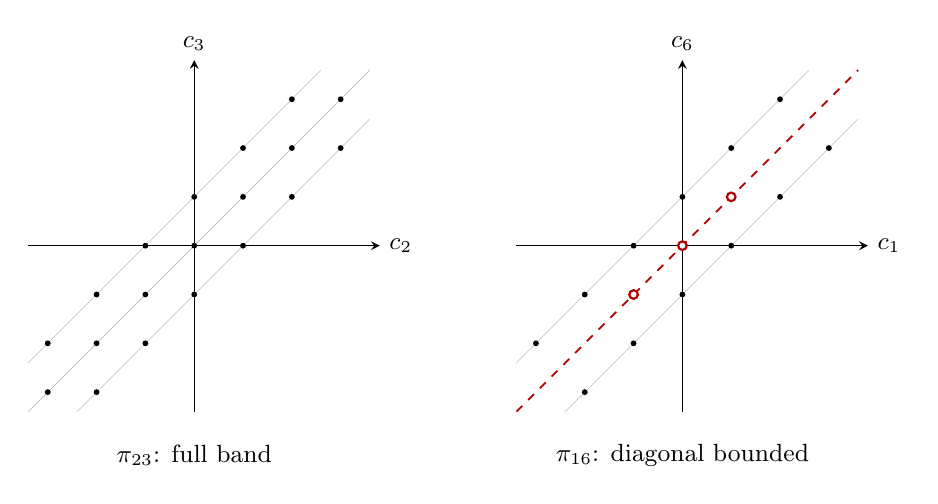
\begin{tikzpicture}[scale=0.62, >=stealth]
  \tikzset{bandline/.style={gray!55, very thin}}
  \begin{scope}
    \draw[bandline] (-2.4,-3.4) -- (3.6,2.6);
    \draw[bandline] (-3.4,-3.4) -- (3.6,3.6);
    \draw[bandline] (-3.4,-2.4) -- (2.6,3.6);
    \draw[->] (-3.4,0) -- (3.8,0) node[right] {\small $c_2$};
    \draw[->] (0,-3.4) -- (0,3.8) node[above] {\small $c_3$};
    \foreach \x in {-3,...,3} {
      \fill (\x,\x) circle (1.7pt);
      \pgfmathtruncatemacro{\xp}{\x+1}
      \ifnum\xp<4 \fill (\xp,\x) circle (1.7pt);\fi
      \pgfmathtruncatemacro{\xm}{\x-1}
      \ifnum\xm>-4 \fill (\xm,\x) circle (1.7pt);\fi
    }
    \node at (0,-4.3) {\small $\pi_{23}$: full band};
  \end{scope}
  \begin{scope}[xshift=10cm]
    \draw[bandline] (-2.4,-3.4) -- (3.6,2.6);
    \draw[red!70!black, dashed, semithick] (-3.4,-3.4) -- (3.6,3.6);
    \draw[bandline] (-3.4,-2.4) -- (2.6,3.6);
    \draw[->] (-3.4,0) -- (3.8,0) node[right] {\small $c_1$};
    \draw[->] (0,-3.4) -- (0,3.8) node[above] {\small $c_6$};
    \foreach \x in {-3,...,3} {
      \pgfmathtruncatemacro{\xp}{\x+1}
      \ifnum\xp<4 \fill (\xp,\x) circle (1.7pt);\fi
      \pgfmathtruncatemacro{\xm}{\x-1}
      \ifnum\xm>-4 \fill (\xm,\x) circle (1.7pt);\fi
    }
    \foreach \x in {-1,0,1} {
      \draw[red!70!black, thick, fill=white] (\x,\x) circle (2.5pt);
    }
    \node at (0,-4.3) {\small $\pi_{16}$: diagonal bounded};
  \end{scope}
\end{tikzpicture}
\caption{Projections of the $c$-vector set of $\widetilde{A}_{2,2}$; the three
band lines $c_v - c_w \in \{-1, 0, 1\}$ are drawn in gray, and the solid dots
mark projected $c$-vectors. For the non-source-sink pair $(2, 3)$ all three lines are
filled. For the source-sink pair $(1, 6)$ the off-diagonal lines are filled,
but the diagonal $c_1 = c_6$ \textup{(}dashed\textup{)} carries only the
bounded regular part: the three open circles at $c_1 = c_6 \in \{-1, 0, 1\}$.}
\label{fig:proj}
\end{figure}

\begin{remark}[Origin]
\label{rem:origin}
The pair $(\widetilde{A}_{2,2}, (1, 6))$ is the squarefree Pr\"ufer
$4$-cycle of Example~\ref{ex:prufer}, the divisor lattice of $6$ under
divisibility, with the bottom $1$ as the source and the top $6$ as the
sink. Theorem~\ref{thm:main} explains, intrinsically, why the
source-sink direction behaves differently from the others: it is the
defect-zero line of the source-sink pair.
\end{remark}

\section{The defect and the congruence criterion}
\label{sec:defect_meaning}

In this section, we separate the two ingredients in projection-filling.
The Auslander--Reiten defect decides which affine root classes are
transjective and hence generate infinite progressions. The common
null-root coordinate decides the step of those progressions and creates a
second, congruence obstruction when it exceeds one. On a source-sink
$\widetilde A_n$ quiver the common coordinate is one and the defect itself
cuts out the non-filled diagonal. In tree type the defect instead decides
whether an already non-filled boundary line is finite or unbounded.

We first isolate the filling criterion underlying
Theorem~\ref{thm:main}, in a form valid in every acyclic simply-laced affine type.

\begin{lemma}[Filling criterion]
\label{lem:filling_criterion}
Let $Q$ be acyclic of affine type and $(v, w)$ a banded pair, that is,
$\delta_v = \delta_w = r$. A band line $\{c_v - c_w = d\}$ is filled if
and only if, for every residue $a \in \ZZ/r\ZZ$, there is a finite root
$\alpha \in \Delta_{\mathrm{fin}}$ such that
\[
  \partial(\alpha) \neq 0, \qquad
  \alpha_v - \alpha_w = d, \qquad
  \alpha_w \equiv a \pmod r.
\]
If a residue is missing, that residue class on the line contains at most
finitely many projected $c$-vectors.
\end{lemma}

\begin{proof}
For every finite root $\alpha$ of nonzero defect, each
$\alpha + m\delta$, $m \in \ZZ$, is a real root of nonzero defect. Its
positive representative is transjective and exceptional; hence
$\alpha + m\delta$ is a signed real Schur root and therefore a $c$-vector.
Its projection is
\[
  \pi_{vw}(\alpha + m\delta)
  = (\alpha_v + mr,\, \alpha_w + mr).
\]
Thus it covers exactly the integer points of the line whose second
coordinate is congruent to $\alpha_w$ modulo $r$. If the displayed
condition holds for every residue, these progressions cover the whole line.

Conversely, write any real root as $\alpha + m\delta$ with
$\alpha \in \Delta_{\mathrm{fin}}$. Its difference and the residue of its
$w$-coordinate are respectively $\alpha_v-\alpha_w$ and
$\alpha_w \bmod r$. If one residue in the statement is not represented by
a finite root of nonzero defect, then no transjective $c$-vector lies in
that residue class on the line. Only regular $c$-vectors can occur there,
and the regular real Schur roots are finite in number. Hence infinitely many
points of that residue class are missing, as desired.
\end{proof}

The role of the defect is now visible, but so is the congruence obstruction.
The defect determines which root classes generate infinite arithmetic
progressions; filling additionally requires those classes to cover every
residue modulo the common null-root coordinate. We record the finiteness of
the regular part intrinsically.

\begin{proposition}[The defect is bounded with finite zero-level]
\label{prop:defect_obstruction}
Let $Q$ be acyclic of affine type. The defect $\partial$ is bounded on
$C(Q)$. Its zero-level $\{c \in C(Q) : \partial(c) = 0\}$ is finite,
consisting of the signed exceptional regular roots, while every nonzero
level of $\partial$ on $C(Q)$ is infinite.
\end{proposition}

\begin{proof}
The defect is invariant under the Auslander--Reiten translate and is
constant on each of the finitely many transjective $\tau$-orbits, so it
takes finitely many values on $C(Q)$. Its zero-level is the set of regular
$c$-vectors, that is, the signed exceptional regular roots; these lie in the
finitely many non-homogeneous tubes and are finite in number, the
homogeneous tubes containing no exceptional modules. Each nonzero value of $\partial$ is
attained on a full transjective $\tau$-orbit, which is infinite, so the
corresponding level is infinite, as desired.
\end{proof}

Thus $\partial$ is the canonical bounded invariant whose vanishing cuts
out the finite regular part. A coordinate projection isolates this finite
part when its difference is the defect. For common null-root coordinate
greater than one, Lemma~\ref{lem:filling_criterion} shows that residue
coverage is an additional requirement.

\begin{theorem}[Projection-filling detects the defect]
\label{thm:defect_detection}
Let $Q$ be acyclic of affine type, and let $(v, w)$ be a banded pair with
$x_v - x_w = \pm\partial$ as linear forms. Then $\pi_{vw}$ fails to fill:
the diagonal $\{c_v - c_w = 0\}$ is the defect-zero locus, and it carries
only the finite regular part of $C(Q)$. For a source-sink orientation of type
$\widetilde{A}_n$, the defect is the coordinate difference
$\partial = (\cdot)_s - (\cdot)_t$, so the hypothesis holds for the
source-sink pair $(s, t)$; there $\partial$ takes only the values $-1, 0, +1$, the band is
$\{|c_s - c_t| \leq 1\}$, the three band lines $c_s - c_t = -1, 0, +1$
are exactly the preprojective, regular, and preinjective strata of
$C(Q)$, and the diagonal is the unique non-filled line. This is the
content of Theorem~\ref{thm:main}.
\end{theorem}

\begin{proof}
If $x_v - x_w = \pm\partial$, then the line $\{c_v - c_w = 0\}$ is the
defect-zero locus, which by Proposition~\ref{prop:defect_obstruction} is
finite, hence unfilled. For a source-sink orientation of type $\widetilde{A}_n$,
Lemma~\ref{lem:defect} gives $\partial = (\cdot)_s - (\cdot)_t$, and
$x_v - x_w = \pm\partial$ holds for a coordinate pair if and only if
$\{v, w\} = \{s, t\}$. Every indecomposable of $\widetilde{A}_n$ has
dimension vector $\alpha_I + m\delta$ with $\alpha_I$ a $0/1$ indicator,
so $\partial(\alpha_I + m\delta) = (\alpha_I)_s - (\alpha_I)_t \in
\{-1, 0, 1\}$, the three values being the preprojective, regular, and
preinjective defects; the band is $\{|c_s - c_t| \leq 1\}$, and the
off-diagonal lines are filled by Theorem~\ref{thm:main}, as desired.
\end{proof}

The point of Theorem~\ref{thm:defect_detection} is that the elementary
combinatorial question of projection-surjectivity recovers a homological
invariant: in the annulus $\widetilde{A}_n$ the unique non-filling
coordinate pair is the one computing the Auslander--Reiten defect
(Theorem~\ref{thm:main}). Off the diagonal, and in other affine types, the
relationship is looser. The next example shows a type where the defect is
not a coordinate difference and every coordinate projection nonetheless
fills; by contrast, in types $\widetilde{E}_7$ and $\widetilde{E}_8$ (and
in $\widetilde{D}_n$ for most acyclic orientations) a projection can fail to fill off the
diagonal (Theorem~\ref{thm:E_classification}), so the defect being a
coordinate difference is \emph{not} necessary for non-filling.

\begin{example}[The obstruction without a non-filling pair: $\widetilde{D}_4$]
\label{ex:D4_meaning}
Let $Q$ be the affine quiver $\widetilde{D}_4$ with central vertex $0$ and
leaves $1, 2, 3, 4$, in the orientation $1 \to 0$, $2 \to 0$, $0 \to 3$,
$0 \to 4$. The null root is $\delta = (2, 1, 1, 1, 1)$, and the defect,
computed as in Lemma~\ref{lem:defect}, is
\[
  \partial \;=\; x_1 + x_2 - x_3 - x_4,
\]
which is \emph{not} a coordinate difference. By
Theorem~\ref{thm:band_dichotomy} the banded pairs are the six leaf-leaf
pairs, each with bound $1$. A direct enumeration of $c$-vectors shows that
\emph{every} leaf-leaf projection fills its band: there is no non-filling
coordinate pair. Yet the defect remains the obstruction in the sense of
Proposition~\ref{prop:defect_obstruction}: on $C(Q)$ it takes the values
$-2, -1, 0, 1, 2$, with the zero-level finite \textup{(}twelve signed
exceptional regular roots\textup{)} and each nonzero level infinite. The
obstruction has simply migrated off the coordinate axes: it lives in the
linear form $\partial$, which no single coordinate projection isolates
because $\partial$ is not a coordinate difference.
\end{example}

\section{Non-filling pairs across affine types}
\label{sec:classification}

In this section, we go beyond the annulus and classify the non-filling
banded pairs completely, over every acyclic orientation of every
simply-laced affine diagram. We first settle every banded pair of null-root
coefficient one (Theorem~\ref{thm:delta_one}): such a pair fills unless it
is the source-sink diagonal of $\widetilde{A}_n$. The
remaining pairs have coefficient at least $2$; for these we develop a short
calculus of box roots (Lemmas~\ref{lem:box} through~\ref{lem:flip}), which
reduces every line to finitely many residue and defect checks, and
we prove the complete classification
(Theorems~\ref{thm:Dtilde_classification}, \ref{thm:E_classification},
and~\ref{thm:complete_classification}): beyond the source-sink diagonals,
non-filling occurs exactly at the width-two boundary lines listed there.
The filling pattern in tree type is orientation-independent; the
orientation controls whether a non-filled boundary is finite or unbounded
through the balanced-geodesic criterion (Remark~\ref{rem:generic}).

Throughout, we write $\ell = x_v - x_w$ for a banded pair $(v, w)$. The
arguments rest on the following spanning property of the hyperplane
$\ker\ell = \{x_v = x_w\}$.

\begin{lemma}[Spanning]
\label{lem:spanning}
Let $Q$ be a connected acyclic quiver of affine type, and let $(v, w)$ be a
pair of distinct vertices. Then the real roots lying on $\ker\ell$ span it.
\end{lemma}

\begin{proof}
The hyperplane $\ker\ell$ has dimension $|Q_0| - 1$, and contains the
$|Q_0| - 2$ linearly independent simple roots $e_i$ with $i \neq v, w$. It
therefore suffices to exhibit one real root on $\ker\ell$ outside their span,
that is, a real root $\alpha$ with $\alpha_v = \alpha_w \neq 0$. The
underlying graph of $Q$ is a tree or a cycle, so it contains a geodesic
$v = u_0, u_1, \dots, u_k = w$ whose vertices induce a subquiver of type
$A_{k+1}$ \textup{(}an induced path: a tree has no chords, and a proper arc
of a cycle is a path\textup{)}. The sum of its simple roots,
$\alpha = \sum_{i=0}^{k} e_{u_i}$, is the highest root of that subsystem,
hence a real root of $Q$, and satisfies $\alpha_v = \alpha_w = 1$. Together
with the $e_i$, $i \neq v, w$, it spans $\ker\ell$, as desired.
\end{proof}

\begin{proposition}[The diagonal detects the defect]
\label{prop:diagonal_defect}
If $\ell = \pm\partial$, then the diagonal line
$\{c_v-c_w=0\}$ contains only the finite regular part and does not fill. If
$\delta_v=\delta_w=1$, the converse also holds: the diagonal fills whenever
$\ell \neq \pm\partial$.
\end{proposition}

\begin{proof}
If $\ell = \pm\partial$, then
$\ker\ell = \ker\partial$ contains no transjective root \textup{(}those
have $\partial \neq 0$\textup{)}; the diagonal therefore contains only the
finite regular part. Now suppose that $\delta_v=\delta_w=1$ and
$\ell \neq \pm\partial$. Were every real root on $\ker\ell$ regular,
then by Lemma~\ref{lem:spanning} the real roots spanning $\ker\ell$ would all
lie in $\ker\partial$, giving $\ker\ell \subseteq \ker\partial$; as both are
hyperplanes this is an equality, so $\partial = c\,\ell$ for a scalar $c$. But
$\ell$ is primitive, and $\partial = \langle\delta, -\rangle$ is primitive as
well \textup{(}the unimodular Euler form sends the primitive null root
$\delta$ to a primitive coefficient vector\textup{)}, so $c = \pm 1$ and
$\ell = \pm\partial$, a contradiction. Hence some real root on $\ker\ell$ is
transjective. Its finite-root representative has difference zero, and the
only residue modulo $\delta_v=1$ is zero; thus the diagonal fills by
Lemma~\ref{lem:filling_criterion}, as desired.
\end{proof}

\begin{corollary}[Coefficient-one diagonals]
\label{cor:diagonal_classification}
A banded coordinate pair $(v, w)$ with
$\delta_v=\delta_w=1$ has a non-filling diagonal if and only if $Q$ is a
source-sink orientation of the $(n+1)$-cycle
\textup{(}type $\widetilde{A}_n$\textup{)} and
$\{v, w\} = \{s, t\}$ is its source-sink pair. In particular such a pair is
unique when it exists.
\end{corollary}

\begin{proof}
By Proposition~\ref{prop:diagonal_defect}, under the coefficient-one
hypothesis a diagonal fails if and only if $\ell = \pm\partial$; i.e., if
and only if $\partial$ is the corresponding coordinate difference. Now
$\partial = \sum_j \partial_j\, x_j$ with
$\partial_j = \delta_j - \sum_{i \to j}\delta_i$ is a coordinate difference
precisely when exactly two coefficients $\partial_j$ are nonzero, equal to
$+1$ and $-1$. For the cycle ($\widetilde{A}_n$), Lemma~\ref{lem:defect}
gives $\partial = \sum_i x_{s_i} - \sum_i x_{t_i}$ over the $k$ sources and
$k$ sinks; this is a coordinate difference if and only if $k = 1$, in
which case
$\partial = x_s - x_t$ is realized by the source-sink pair, while an
orientation with $k \geq 2$ has $2k \geq 4$ nonzero coefficients and no
failing diagonal. For trees we count nonzero coefficients by leaves: at a
leaf $j$ with unique neighbor $k$, the null-root relation $2\delta_j =
\sum_{i \sim j}\delta_i$ gives $\delta_k = 2\delta_j$, so $\partial_j =
\delta_j$ if $j$ is a source and $\partial_j = \delta_j - \delta_k =
-\delta_j$ if $j$ is a sink; thus $\partial_j = \pm\delta_j \neq 0$ at
\emph{every} leaf, in any orientation. Types $\widetilde{D}$ and
$\widetilde{E}$ are trees with at least three leaves \textup{(}four for
$\widetilde{D}_n$, three for $\widetilde{E}_n$\textup{)}, so $\partial$ has
at least three nonzero coefficients and is not a coordinate difference. The
stated classification follows, as desired.
\end{proof}

\begin{remark}[Seed-dependence of the filling pattern]
\label{rem:seed_dependence}
The $c$-vector set $C(Q)$, and with it the filling pattern, depends on the
chosen acyclic seed, not merely on its mutation type. On the $4$-cycle with
vertices $\{0, 1, 2, 3\}$ the source-sink orientation $0 \to 1 \to 2$,
$0 \to 3 \to 2$ has defect $x_0 - x_2$ and the unique non-filling pair
$(0, 2)$ of Theorem~\ref{thm:main}, whereas the alternating orientation
$0 \to 1 \leftarrow 2 \to 3 \leftarrow 0$ has two sources $\{0, 2\}$ and two
sinks $\{1, 3\}$, defect $\partial = x_0 - x_1 + x_2 - x_3$ \textup{(}not a
coordinate difference\textup{)}, and hence no non-filling pair at all, by
Theorem~\ref{thm:delta_one} \textup{(}the diagonal case being
Corollary~\ref{cor:diagonal_classification}\textup{)}. Both are of cluster type
$\widetilde{A}_{2, 2}$, the type of the Pr\"ufer example
\textup{(}Example~\ref{ex:prufer}\textup{)}; so non-filling is a property of
the source-sink seed, not of the annulus cluster algebra in the abstract.
This is why we fix the source-sink orientation throughout.
\end{remark}

We next bound the regular contribution to any band; it confines all further
non-filling to pairs of null-root coefficient at least $2$.

\begin{lemma}[Regular band bound]
\label{lem:regular_bound}
Let $(v, w)$ be a banded pair, so $\delta_v = \delta_w$. Every regular
$c$-vector $c$ satisfies $|c_v - c_w| \leq \delta_v$. In particular a band line
$\{c_v - c_w = d\}$ with $|d| \geq 2$ that is met by a regular $c$-vector
forces $\delta_v = \delta_w \geq 2$.
\end{lemma}

\begin{proof}
A regular $c$-vector is, up to sign, the dimension vector of an exceptional
regular module: the positive $c$-vectors are the real Schur roots
(\S\ref{sec:prelim}), a regular one is a real Schur root of vanishing defect,
and such a root is the dimension vector of an exceptional regular
indecomposable. Write the $c$-vector as $\pm\beta$ with $\beta = \underline{\dim}\,M$;
it suffices to prove $0 \leq \beta \leq \delta$ componentwise, since then both
$\beta_v$ and $\beta_w$ lie in $[0, \delta_v]$ (using $\delta_w = \delta_v$),
so $|c_v - c_w| = |\beta_v - \beta_w| \leq \delta_v$.

We recall the structure of the regular components
\textup{(}\cite[\S3]{Ringel1984}\textup{)}. The regular indecomposables lie
in tubes; in a tube of rank $r$ the quasi-simple objects
$S_1, \dots, S_r$, cyclically ordered, are its regular simple modules, and
their dimension vectors satisfy $\sum_{i=1}^{r} \underline{\dim}\,S_i =
\delta$. Every indecomposable of the tube is uniserial for the regular
composition series, determined by its quasi-socle $S_j$ and quasi-length
$m \geq 1$, with quasi-composition factors the $m$ consecutive quasi-simples
$S_j, S_{j+1}, \dots, S_{j+m-1}$ \textup{(}indices modulo $r$\textup{)}; hence
\[
  \beta \;=\; \underline{\dim}\,M \;=\; \sum_{i=0}^{m-1} \underline{\dim}\,S_{\,j+i}.
\]
By the preliminaries the exceptional regular indecomposables are exactly
those of quasi-length $m \leq r - 1$; since $M$ is exceptional we have
$1 \leq m \leq r - 1$, so in particular $r \geq 2$ and the tube is
non-homogeneous. The $m$ summands are then pairwise distinct quasi-simples
\textup{(}being fewer than a full cycle of length $r$\textup{)}, so the
complementary $r - m \geq 1$ quasi-simples form the disjoint consecutive arc
$S_{j+m}, \dots, S_{j+r-1}$, and
\[
  \delta - \beta \;=\; \sum_{i=m}^{r-1} \underline{\dim}\,S_{\,j+i}
\]
is again a sum of dimension vectors of modules, hence nonnegative. Both $\beta$ and $\delta -
\beta$ are therefore nonnegative in every coordinate, that is,
$0 \leq \beta \leq \delta$, as required.

For the last assertion, if a regular $c$-vector $c$ meets the line $c_v - c_w =
d$, then $|d| = |c_v - c_w| \leq \delta_v = \delta_w$ by the bound just
proved, so $|d| \geq 2$ forces $\delta_v = \delta_w \geq 2$, as desired.
\end{proof}

A second ingredient identifies the coefficient-one vertices outside the
cycle.

\begin{lemma}[Coefficient one forces a leaf]
\label{lem:mark_one_leaf}
Let $Q$ be a connected acyclic quiver of affine type whose underlying graph
is a tree. If $\delta_v = 1$, then $v$ is a leaf.
\end{lemma}

\begin{proof}
The null root spans the radical of the symmetric Tits form, so it satisfies
the balance relation $2\delta_v = \sum_{u \sim v}\delta_u$ at every vertex
$v$. Let $T = \{u : \delta_u = 1,\ \deg u \geq 2\}$; we show $T =
\varnothing$, which is the claim. Suppose $v \in T$. Since $\sum_{u \sim v}
\delta_u = 2\delta_v = 2$ and each $\delta_u \geq 1$, the vertex $v$ has
exactly two neighbors, both of coefficient $1$. For such a neighbor $u$ one
has $\delta_u = 1$; were $\deg u = 1$, its unique neighbor would be $v$ and
the balance relation would read $2 = 2\delta_u = \delta_v = 1$, which is
absurd. So $\deg u \geq 2$ and $u \in T$. Thus every vertex of $T$ has both
of its neighbors in $T$, so the subgraph induced on $T$ is $2$-regular and
contains a cycle. As $Q$ is a tree this is impossible, so $T = \varnothing$
and every coefficient-one vertex is a leaf, as desired.
\end{proof}

With these in hand we settle every banded pair of coefficient one.

\begin{theorem}[Coefficient-one pairs fill]
\label{thm:delta_one}
Let $Q$ be a connected acyclic quiver of affine type, and let $(v, w)$ be a
banded pair with $\delta_v = \delta_w = 1$. Then $\pi_{vw}$ surjects onto the
whole band, unless $Q$ is a source-sink orientation of the $(n+1)$-cycle and
$(v, w)$ is its source-sink pair, in which case the diagonal $\{c_v = c_w\}$
is the only band line that fails to fill.
\end{theorem}

\begin{proof}
If $Q$ is a source-sink orientation of the $(n+1)$-cycle, this is
Theorem~\ref{thm:main}. If $Q$ is any other orientation of the cycle, it has
$k \geq 2$ sources, so by Lemma~\ref{lem:defect} its defect has $2k \geq 4$
nonzero coefficients and is not a coordinate difference; the diagonal $d = 0$
then fills by Corollary~\ref{cor:diagonal_classification}. For $d = +1$ we
exhibit a transjective cyclic interval containing $v$ but not $w$: if $v$ is a
source or a sink, the singleton $\{v\}$ is such an interval
\textup{(}defect $\pm 1$\textup{)}; otherwise $v$ is interior to a maximal
directed arc bounded by a source $s$ and a sink $t$, and the sub-arcs from $s$
to $v$ and from $v$ to $t$ each contain exactly one of $\{s, t\}$, hence are
transjective, and meet only in $v$, so the one avoiding $w$ is the desired
interval. Its $\delta$-shifts fill $\{c_v - c_w = 1\}$, and the sign $-1$
fills $\{c_v - c_w = -1\}$. Since $\delta = (1, \dots, 1)$, the band is
$\{|c_v - c_w| \leq 1\}$ by Theorem~\ref{thm:band_dichotomy}, so these are all
its lines and every one fills. Finally suppose $Q$ is a tree. Every
positive finite root satisfies $\alpha \leq \theta \leq \delta$, where
$\theta$ is the highest root of $\Delta_{\mathrm{fin}}$ and $\delta =
\theta + e_{v_0}$ at the extending vertex $v_0$, so $|\alpha_v -
\alpha_w| \leq \delta_v = 1$ and the band is $\{|c_v - c_w| \leq 1\}$ by
Theorem~\ref{thm:band_dichotomy}; it remains to treat $d = -1, 0, 1$.

By Lemma~\ref{lem:mark_one_leaf} both $v$ and $w$ are leaves. A leaf is a
source or a sink of $Q$, so its simple module is injective or projective,
hence preinjective or preprojective; in particular the simple root $e_v$ is
transjective \textup{(}$\partial(e_v) = \pm 1 \neq 0$\textup{)}, and likewise
$e_w$. By Lemma~\ref{lem:box_schur}, the signed shift families
$e_v + m\delta$ and $e_w + m\delta$, $m \in \ZZ$, project onto every
integer point of the lines $\{c_v-c_w=1\}$ and
$\{c_v-c_w=-1\}$, respectively. Finally, by the computation in the proof of
Corollary~\ref{cor:diagonal_classification} the defect $\partial$ is a
coordinate difference only for the source-sink pair of the cycle; as $Q$ is a
tree, $\partial \neq \pm(x_v - x_w)$, so the diagonal $d = 0$ fills by
Proposition~\ref{prop:diagonal_defect}. Hence the whole band fills, as
desired.
\end{proof}

In particular, among banded pairs with $\delta_v = \delta_w = 1$ the only
failure is the source-sink diagonal of $\widetilde{A}_n$; this resolves all
of type $\widetilde{A}_n$ together with every leaf-leaf pair of
$\widetilde{D}$ and $\widetilde{E}$. The remaining banded pairs have
$\delta_v = \delta_w \geq 2$, where congruence classes become nontrivial
and Lemma~\ref{lem:regular_bound} confines the regular contribution. For the
rest of this section the underlying graph of $Q$ is therefore a tree, $(v,
w)$ is a banded pair with $\delta_v = \delta_w \geq 2$, and we write
$\ell(x) = x_v - x_w$ as before. We call a positive real root $\beta$ with
$\beta \leq \delta$ componentwise a \emph{box root} and refer to
$\ell(\beta)$ as its \emph{level}. Observe that the box roots, their levels,
and the banded pairs themselves do not depend on the orientation of $Q$,
whereas the defect does; the classification is exactly the interplay of the
two.

\begin{lemma}[Box representatives]
\label{lem:box}
The box roots are exactly the elements of
$\Delta_{\mathrm{fin}}^{+} \sqcup (\delta - \Delta_{\mathrm{fin}}^{+})$,
and every positive real root is $\beta + m\delta$ for a unique box root
$\beta$ and a unique integer $m \geq 0$. Moreover, for a banded pair
$(v, w)$:
\begin{enumerate}[label=\textup{(\arabic*)}]
\item writing $r=\delta_v=\delta_w$, a band line
  $\{c_v-c_w=d\}$ is filled if and only if, for every
  $a\in\ZZ/r\ZZ$, some box root $\beta$ satisfies
  \[
    \ell(\beta)=d,\qquad \beta_w\equiv a\pmod r,
    \qquad \partial(\beta)\neq0;
  \]
\item the set of differences $c_v - c_w$ realized on $C(Q)$ is exactly
  the set of levels of box roots.
\end{enumerate}
\end{lemma}

\begin{proof}
By the preliminaries the positive real roots are the $\alpha + m\delta$ with
$\alpha \in \Delta_{\mathrm{fin}}^{+}$ and $m \geq 0$, together with the
$-\alpha + m\delta$ with $m \geq 1$; the latter is $(\delta - \alpha) +
(m-1)\delta$. Both $\alpha$ and $\delta - \alpha$ lie in the box: a positive
finite root satisfies $\alpha \leq \theta \leq \delta$, where $\theta$ is
the highest root of $\Delta_{\mathrm{fin}}$ and $\delta = \theta + e_{v_0}$
for the extending vertex $v_0$. The two families are disjoint, since
$\alpha = \delta - \alpha'$ would force $\alpha + \alpha' = \delta$, which
is impossible at the extending vertex, where finite roots vanish; and
$(\beta, m)$ is unique because two box vectors cannot differ by a nonzero
multiple of $\delta$.

For (1), the box roots give one representative of every signed real-root
class modulo $\ZZ\delta$. A box root of nonzero defect generates, by
Lemma~\ref{lem:box_schur}, exactly one residue class modulo $r$ on its band
line. The assertion is therefore the box-root form of
Lemma~\ref{lem:filling_criterion}.

For (2), every $c$-vector is $\pm(\beta + m\delta)$, so its difference
$c_v - c_w$ is $\pm\ell(\beta)$; here we use $\delta_v = \delta_w$.
The negative value is also a box-root level because
$\ell(\delta-\beta)=-\ell(\beta)$. Conversely every box root is a $c$-vector by
Lemma~\ref{lem:box_schur}. Hence every level is attained by a $c$-vector,
as desired.
\end{proof}

\begin{lemma}[Low levels fill]
\label{lem:low_levels}
For every orientation of $Q$, the lines $c_v - c_w \in \{-1, 0, 1\}$ are
filled.
\end{lemma}

\begin{proof}
First suppose that $Q$ has type $\widetilde D_n$. Then $v$ and $w$ are
spine vertices and $r=\delta_v=\delta_w=2$. Choose a leaf $z$ on the
$v$-side of the spine, so that the path from $v$ to $z$ avoids $w$. The
indicators of the successive prefixes of this path are box roots of level
$1$ and have $w$-coordinate $0$. At least one has nonzero defect: otherwise
successive differences would give $\partial(e_z)=0$, whereas every leaf has
defect coefficient $\pm1$. This supplies residue $0$ modulo $2$ on the line
of level $1$. Applying the same argument from $w$ to a leaf on the
$w$-side gives a transjective path root $\gamma$ of level $-1$ with
$\gamma_w=1$. Its mirror $\delta-\gamma$ has level $1$, nonzero defect, and
$w$-coordinate $1$ modulo $2$. Lemma~\ref{lem:box}(1) now fills the line of
level $1$; interchanging $v$ and $w$ fills the line of level $-1$.

For the diagonal, a leaf simple root distinct from $v,w$ supplies residue
$0$. To obtain residue $1$, start with the indicator of the path from $v$
to $w$ and extend it, one vertex at a time, from $v$ toward a leaf on the
$v$-side. All these path roots have level $0$ and $w$-coordinate $1$. If
all had defect zero, their successive differences would again force the
leaf simple root to have defect zero. Hence one is transjective, and the
diagonal fills.

For the three exceptional tree types the remaining assertion is a finite
exact check. For every orientation, every banded pair of common coefficient
at least $2$, every $d\in\{-1,0,1\}$, and every residue modulo that
coefficient, we enumerate the vectors $0<\beta\leq\delta$ and retain those
with $q(\beta)=1$, level $d$, the prescribed residue, and nonzero defect.
The numbers of obligations checked are
\[
\begin{array}{c|c|c}
\text{type} & \text{orientations} &
\text{(orientation, pair, level, residue) obligations}\\ \hline
\widetilde E_6 & 64 & 1152\\
\widetilde E_7 & 128 & 3456\\
\widetilde E_8 & 256 & 6912
\end{array}
\]
and every obligation has a witness. The computation is exact integer
arithmetic and is reproduced by the ancillary certificate described in
Remark~\ref{rem:computation}. Lemma~\ref{lem:box}(1) therefore gives the
three filled lines in every exceptional type, as desired.
\end{proof}

\begin{lemma}[Flip lemma]
\label{lem:flip}
Let $Q'$ be obtained from $Q$ by reversing a single arrow $a \to b$, and
let $\beta$ be any vector. Then
\[
  \partial_{Q'}(\beta) \;=\; \partial_{Q}(\beta) + \delta_a \beta_b -
  \delta_b \beta_a.
\]
In particular the value $\partial(\beta)$ depends only on the orientations
of the edges $\{a, b\}$ with $\delta_a \beta_b \neq \delta_b \beta_a$,
which we call the edges \emph{relevant to} $\beta$.
\end{lemma}

\begin{proof}
We have $\partial(\beta) = \langle \delta, \beta \rangle = \sum_i \delta_i
\beta_i - \sum_{i \to j} \delta_i \beta_j$, and the reversal replaces the
term $-\delta_a \beta_b$ by $-\delta_b \beta_a$, as desired.
\end{proof}

By Lemma~\ref{lem:box}(2) the differences realized on $C(Q)$ are exactly
the levels of box roots. In
type $\widetilde{D}_n$ every coordinate of $\delta$ is at most $2$, so
every level satisfies $|\ell(\beta)| \leq 2$; in types $\widetilde{E}_6,
\widetilde{E}_7, \widetilde{E}_8$ the same bound holds for every box root
and banded pair, by inspection of the finitely many positive roots
(Remark~\ref{rem:computation}). Combined with Lemma~\ref{lem:low_levels},
the classification is reduced to the boundary levels $\pm2$. We call the
box roots of level $2$ the \emph{extremal roots} of the pair. Their
coordinates determine which congruence classes occur on a boundary line,
while their defects determine whether those classes are infinite or only
regular and finite.

We begin with the one infinite family, type $\widetilde{D}_n$, where the
classification is uniform in $n$ and in the orientation.

\begin{theorem}[Type $\widetilde{D}_n$, all orientations]
\label{thm:Dtilde_classification}
Let $Q$ be any orientation of the $\widetilde{D}_n$ diagram, $n \geq 4$:
spine vertices $u_1, \dots, u_{n-3}$ of null-root coefficient $2$, two
leaves attached to $u_1$ and two to $u_{n-3}$. The leaf pairs and adjacent
spine pairs fill their bands. Every spine pair $(u_a,u_b)$ at distance
$b-a\geq2$ has band $|c_{u_a}-c_{u_b}|\leq2$, and its two boundary lines
$c_{u_a}-c_{u_b}=\pm2$ do not fill. More precisely:
\begin{enumerate}[label=\textup{(\arabic*)}]
\item if $b-a=2$ and the middle vertex $u_{a+1}$ is a source or a sink,
  each boundary line contains only finitely many regular $c$-vectors;
\item otherwise each boundary line contains an infinite arithmetic
  progression of transjective $c$-vectors, but the other parity class
  contains only finitely many regular $c$-vectors.
\end{enumerate}
\end{theorem}

\begin{proof}
The leaf pairs have coefficient $1$ and are settled by
Theorem~\ref{thm:delta_one}, so let $(v, w) = (u_a, u_b)$ with $a < b$ be a
spine pair, and write $d = b - a$. By Lemma~\ref{lem:low_levels} the lines
$0, \pm 1$ fill, and every level is at most $2$ in absolute value.

We first list the extremal roots. In the standard realization of $D_n$, the
positive roots are the vectors $e_i-e_j$ and $e_i+e_j$ with $i<j$.
Expressing these vectors in the simple-root basis on the diagram, and then
including the mirrors $\delta-\alpha$ from Lemma~\ref{lem:box}, shows that
the box roots with coordinates $(2,0)$ at $(u_a,u_b)$ are exactly
\[
  \beta_{p, q} \;=\; e_{\ell_1} + e_{\ell_2} + 2(e_{u_1} + \dots + e_{u_p})
  + (e_{u_{p+1}} + \dots + e_{u_q}),
  \qquad a \leq p < q \leq b - 1,
\]
where $\ell_1, \ell_2$ are the two leaves at $u_1$. Indeed, the
$e_i-e_j$ roots become path indicators and cannot have level $2$; among the
$e_i+e_j$ roots, the displayed simple-root expansion has a $2$-string
through $u_a$ and ends its following $1$-string before $u_b$ exactly for the
listed indices. An expansion anchored at the other fork with level $-2$ has
its mirror among the displayed vectors; every remaining expansion and its
mirror has level at most $1$ in absolute value. This exhausts the standard
root list. In particular there is no extremal root when
$d = 1$, at least one when $d\geq2$, and exactly one when $d = 2$, namely
$\beta^{*} = \beta_{a, a+1}$. Thus adjacent spine pairs have width one and
fill by Lemma~\ref{lem:low_levels}. If $d\geq2$, every extremal root has
coordinates $(2,0)$ at $(u_a,u_b)$. Its $\delta$-shifts therefore cover
only the even residue on the line of level $2$; the odd residue contains
only finitely many regular $c$-vectors. The mirror statement gives the same
conclusion at level $-2$. Hence neither boundary line fills, by
Lemma~\ref{lem:box}(1), regardless of orientation.

Suppose $d = 2$. By the flip lemma the only edges relevant to $\beta^{*}$
are the two spine edges at the middle vertex $u_{a+1}$: along the
$2$-string and the $0$-string the products $\delta_x \beta^{*}_y$ and
$\delta_y \beta^{*}_x$ agree, as they do on the four leaf edges
\textup{(}$1 \cdot 2 = 2 \cdot 1$ at the near fork, $0 = 0$ at the
far\textup{)}. For any orientation with $u_a \to u_{a+1} \to u_{a+2}$ a
direct evaluation gives $\partial(\beta^{*}) = 2$, and by
Lemma~\ref{lem:flip} reversing the arrow $u_a \to u_{a+1}$, respectively
$u_{a+1} \to u_{a+2}$, changes the value by $2 \cdot 1 - 2 \cdot 2 = -2$,
respectively $2 \cdot 0 - 2 \cdot 1 = -2$. Hence $\partial(\beta^{*}) =
\pm 2 \neq 0$ when the two spine arrows at $u_{a+1}$ point the same way
along the spine, and $\partial(\beta^{*}) = 0$ when $u_{a+1}$ is a source
or a sink. In the latter case the boundary lines carry only the finite
regular part; otherwise the extremal class supplies the infinite even
progression asserted in part~\textup{(}2\textup{)}.

Suppose $d \geq 3$, and suppose to the contrary that every extremal root
$\beta_{p, q}$, $a \leq p < q \leq b - 1$, has defect $0$. Taking
differences,
\[
  \partial(e_{u_{q+1}}) = \partial(\beta_{p, q+1}) - \partial(\beta_{p, q})
  = 0
  \quad\text{and}\quad
  \partial(e_{u_{p+1}}) = \partial(\beta_{p+1, q}) - \partial(\beta_{p, q})
  = 0
\]
for all admissible indices, so $\partial(e_{u_k}) = 0$ for every $k$ with
$a < k < b$. For such an interior spine vertex we have $\partial(e_{u_k}) =
\delta_{u_k} - \sum_{i \to u_k} \delta_i = 2 - 2 \cdot \#\{\text{arrows
into } u_k\}$, which vanishes exactly when $u_k$ has one arrow in and one
arrow out. Thus no $u_k$ with $a < k < b$ is a source or a sink; but then
the $d = 2$ computation gives $\partial(\beta_{a, a+1}) = \pm 2 \neq 0$, a
contradiction. Hence some extremal root is transjective and each boundary
line contains an infinite arithmetic progression. The residue argument
above shows that it nevertheless does not fill, which finishes the proof.
\end{proof}

We turn to the three exceptional types, where the box roots form a finite,
orientation-independent list and the same calculus applies verbatim.

\begin{theorem}[Types $\widetilde{E}_6$, $\widetilde{E}_7$,
$\widetilde{E}_8$, all orientations]
\label{thm:E_classification}
Let $Q$ be any orientation of a diagram of type $\widetilde{E}_6$,
$\widetilde{E}_7$, or $\widetilde{E}_8$. Then:
\begin{enumerate}[label=\textup{(\arabic*)}]
\item in $\widetilde{E}_6$, every banded pair fills;
\item in $\widetilde{E}_7$, with central vertex $0$, short arm $1$, and
  long arms $2, 3, 4$ and $5, 6, 7$ \textup{(}listed outward\textup{)},
  every banded pair fills except $(3, 6)$. Its lines $\pm 2$ never fill;
  they are finite exactly when the geodesic $3, 2, 0, 5, 6$ carries two
  arrows in each direction, and otherwise each contains an infinite
  arithmetic progression;
\item in $\widetilde{E}_8$, with central vertex $0$ and arms $1$; $2, 3$;
  $4, 5, 6, 7, 8$ \textup{(}listed outward\textup{)}, every banded pair
  fills except $(1, 6)$, $(2, 5)$, and $(3, 7)$. Their lines $\pm2$ never
  fill. For $(1,6)$ they are finite exactly when the geodesic
  $1,0,4,5,6$ is balanced, and for $(3,7)$ exactly when
  $3,2,0,4,5,6,7$ is balanced. For $(2,5)$ the geodesic has odd length,
  so each boundary line always contains an infinite arithmetic progression.
\end{enumerate}
Whenever one of these boundary lines is infinite, it still misses all but
finitely many points in at least one residue class modulo the common
null-root coordinate.
\end{theorem}

\begin{proof}
The null roots in the three cases are
\[
  \delta = (3;\, 2, 1;\, 2, 1;\, 2, 1), \qquad
  (4;\, 2;\, 3, 2, 1;\, 3, 2, 1), \qquad
  (6;\, 3;\, 4, 2;\, 5, 4, 3, 2, 1),
\]
the central coordinate listed first. Coefficient-one pairs fill by
Theorem~\ref{thm:delta_one}, and the lines $0, \pm 1$ of every banded pair
fill by Lemma~\ref{lem:low_levels}, so by Lemma~\ref{lem:box} only the
extremal roots of the coefficient-$\geq 2$ pairs are in question.
Enumerating the finitely many box roots, an exact and
orientation-independent computation (Remark~\ref{rem:computation}), yields:
in $\widetilde{E}_6$ no banded pair has an extremal root, so every band is
$\{|c_v - c_w| \leq 1\}$ and fills; in $\widetilde{E}_7$ the only pair with
an extremal root is $(3, 6)$, and in $\widetilde{E}_8$ the pairs with
extremal roots are $(1, 6)$, $(2, 5)$, and $(3, 7)$; each has a unique
one, namely
\begin{gather*}
  \beta^{*}_{(3,6)} = (2; 1; 2, 2, 1; 1, 0, 0), \qquad
  \beta^{*}_{(1,6)} = (3; 2; 2, 1; 2, 1, 0, 0, 0), \\
  \beta^{*}_{(2,5)} = (2; 1; 2, 1; 1, 0, 0, 0, 0), \qquad
  \beta^{*}_{(3,7)} = (4; 2; 3, 2; 3, 2, 1, 0, 0).
\end{gather*}
For every displayed pair, the extremal root has
$(\beta_v^{*},\beta_w^{*})=(2,0)$. Since it is the unique box root of level
$2$, transjective shifts can cover at most residue $0$ modulo the common
null-root coordinate. The mirror root gives the same conclusion at level
$-2$. Thus all four pairs have non-filled boundary lines, independently of
orientation; the defect decides whether those lines are finite or
unbounded.

In each case one checks $\delta_x \beta^{*}_y = \delta_y \beta^{*}_x$ on
every edge $\{x, y\}$ off the geodesic from $v$ to $w$, so by the flip
lemma the edges relevant to $\beta^{*}$ are exactly the geodesic edges.
Writing $f$ and $b$ for the numbers of geodesic arrows pointing with,
respectively against, the walk from $v$ to $w$, the value at one reference
orientation together with the flip increments of Lemma~\ref{lem:flip}
determines the affine function $\partial(\beta^{*})$ completely, and a
direct evaluation gives
\[
  \bigl|\partial(\beta^{*})\bigr| \;=\; c \, |f - b|.
\]
Here $c=1, \tfrac{3}{2}, 2, 1$ for the pairs $(3,6)$, $(1,6)$, $(2,5)$,
$(3,7)$, respectively; every flip increment has magnitude $2c$, aligned with the
walk. Hence $\partial(\beta^{*}) = 0$ if and only if $f = b$. For $(2, 5)$
the geodesic $2, 0, 4, 5$ has odd length, so $f \neq b$ for every
orientation and the boundary lines are always unbounded. For $(3, 6)$,
$(1, 6)$, and $(3, 7)$ the geodesics have lengths $4$, $4$, and $6$;
$f=b$ is exactly the stated finiteness criterion. When equality holds only
the finite regular part remains on the boundary, while otherwise the
extremal class supplies an infinite arithmetic progression, as desired.
\end{proof}

Assembling the pieces yields the complete classification.

\begin{theorem}[The complete classification]
\label{thm:complete_classification}
Let $Q$ be a connected acyclic quiver of simply-laced affine type, in any
orientation, and let $(v, w)$ be a banded pair. Then $\pi_{vw}$ surjects onto its band,
with exactly two families of exceptions:
\begin{enumerate}[label=\textup{(\arabic*)}]
\item \textup{(interior gap)} $Q$ is a source-sink orientation of a cycle
  and $(v, w)$ is its source-sink pair; the unique non-filled line is the
  diagonal $c_v - c_w = 0$;
\item \textup{(boundary congruence gap)} $Q$ has tree type and $(v,w)$ is
  one of the following extremal pairs: two spine vertices at distance at
  least two in $\widetilde D_n$; the pair $(3,6)$ in $\widetilde E_7$; or
  one of $(1,6)$, $(2,5)$, $(3,7)$ in $\widetilde E_8$. The two non-filled
  lines are $c_v-c_w=\pm2$.
\end{enumerate}
In the second family, a boundary line is finite exactly in the balanced
unique-extremal-root cases: a distance-two $\widetilde D_n$ pair whose
middle vertex is a source or a sink, or one of $(3,6)$ in
$\widetilde E_7$ and $(1,6),(3,7)$ in $\widetilde E_8$ with balanced
geodesic. Every other non-filled boundary line contains an infinite
arithmetic progression but misses a residue class modulo
$\delta_v=\delta_w$.
\end{theorem}

\begin{proof}
For the cycle, Theorem~\ref{thm:delta_one} and
Corollary~\ref{cor:diagonal_classification} leave exactly the source-sink
diagonals of Theorem~\ref{thm:main}. For the trees, coefficient-one pairs
are settled by Theorem~\ref{thm:delta_one}, and the coefficient-$\geq 2$
pairs by Theorems~\ref{thm:Dtilde_classification}
and~\ref{thm:E_classification}. For a distance-two spine pair the geodesic
consists of the two spine edges at the middle vertex, which is balanced
exactly when one arrow points each way; i.e., when the middle vertex is a
source or a sink. The finite-versus-unbounded refinement is therefore
exactly the one stated in those two theorems, as desired.
\end{proof}

\begin{remark}[Genericity and seed-dependence]
\label{rem:generic}
Theorem~\ref{thm:complete_classification} makes the seed-dependence of
Remark~\ref{rem:seed_dependence} more precise. Filling itself is
orientation-independent in tree type: every orientation of
$\widetilde D_n$, $n\geq6$, has a non-filling spine pair, every orientation
of $\widetilde E_7$ has the non-filling pair $(3,6)$, and every orientation
of $\widetilde E_8$ has the three non-filling pairs listed above. What
depends on the orientation is whether a non-filled boundary line is finite
or unbounded. In $\widetilde D_n$, exactly $32$ of the $2^n$ orientations
have no finite boundary line: the two directed-spine orientations with the
four leaf edges free. Thus the other $2^n-32$ orientations have at least one
finite boundary line. Similarly, $48$ of the $128$ orientations of
$\widetilde E_7$ and $140$ of the $256$ orientations of
$\widetilde E_8$ have at least one finite boundary line. By contrast,
$\widetilde D_4$, $\widetilde D_5$, and $\widetilde E_6$ fill for every
orientation.
\end{remark}

\begin{remark}[Computational verification]
\label{rem:computation}
The classification is verified by the fail-closed ancillary certificate
\path{anc/verify_residue_classification.py}. It enumerates the box roots
once for each underlying graph and then sweeps every orientation: cycles on
up to $7$ vertices, $\widetilde D_n$ for $n\leq13$, and all three
exceptional types. For each banded pair and level it records not only the
difference but also the residue of one coordinate modulo
$r=\delta_v=\delta_w$, exactly as required by Lemma~\ref{lem:box}(1). It
also checks the extremal-root lists, the balanced-geodesic criterion, and
the orientation counts in Remark~\ref{rem:generic}. Every load-bearing test
uses Python integer and rational arithmetic: box roots satisfy
$q(\beta)=1$ over $\ZZ$, and defects are the exact integers
$\langle\delta,\beta\rangle$. The older mutation and Coxeter scripts are
retained only as finite spot checks and are not used to prove absence or
surjectivity. The ancillary README gives the command and expected
certificate hash.
\end{remark}

In summary, non-filling falls under two headings: the defect-zero diagonal
of a source-sink affine cycle, and a congruence gap on the boundary of a
width-two tree-type band. The second mechanism persists even when the
boundary contains infinitely many transjective roots, because a
$\delta$-shift advances both projected coordinates by
$r=\delta_v=\delta_w$ and therefore preserves their residue modulo $r$.
The defect supplies a finer dichotomy inside this non-filling family: a
balanced extremal class is regular and leaves a finite boundary line,
whereas a nonzero-defect class generates an infinite arithmetic progression
without filling the missing residues.

\section{The annulus as a surface: defect and Dehn twist}
\label{sec:surface}

In this section, we make the topological reading of Theorem~\ref{thm:main}
precise: on the annulus, the trichotomy
preprojective/regular/preinjective becomes the dichotomy
bridging/peripheral together with a sign, the absolute defect is the
crossing number with the core curve, and the $\delta$-shift is the Dehn twist along
it. This places the filling theorem in the line of geometric descriptions
of $c$-vectors by non-self-crossing curves on surfaces
\textup{(}\cite{FominShapiroThurston2008, Hong2021}; conjecturally in
general \cite{LeeLeeMills2019}\textup{)}.

Let $C_{p, q}$ denote the annulus with $p$ marked points on the outer
boundary and $q$ on the inner, $p + q = n + 1$, and let $c$ be its core
curve. We work in the universal cover: identify the outer marked points
with $\ZZ$ \textup{(}reduction mod $p$\textup{)} and the inner marked
points with $\ZZ$ \textup{(}reduction mod $q$\textup{)}, the deck
transformation acting by $(a, b) \mapsto (a + p, b + q)$. An arc is
\emph{bridging} if it joins the two boundary components and
\emph{peripheral} otherwise; a bridging arc is determined by an endpoint
pair $(a, b)$ up to the deck action, and two bridging arcs $(a, b)$ and
$(a', b')$ have minimal crossing number
\[
  i\bigl((a, b), (a', b')\bigr)
  \;=\; \#\{\, k \in \ZZ : (a - a' - kp)(b - b' - kq) < 0 \,\}.
\]
Let $T$ be the \emph{fan} triangulation, with bridging arcs $(j, 0)$ for
$0 \leq j \leq p$ and $(p, j)$ for $1 \leq j \leq q - 1$. Every triangle
of $T$ has a side on a boundary: $p$ triangles on the outer boundary and
$q$ on the inner. The arrows of the adjacency quiver of $T$ run
consistently along the outer fan and consistently along the inner fan, so
the quiver is the source-sink orientation of the $(n+1)$-cycle, with $s$
and $t$ the two arcs shared by the outer and the inner fan. We use the
standard dictionary for triangulated unpunctured surfaces
\textup{(}\cite{FominShapiroThurston2008, ABCP2010, BrustleZhang2011}; the
modules here are string modules in the sense of
\cite{ButlerRingel1987}\textup{)} in the
following form: the assignment $\gamma \mapsto M_\gamma$, where
$(\underline{\dim}\, M_\gamma)_i$ is the minimal crossing number of
$\gamma$ with $\tau_i$, is a bijection between the essential arcs of
$C_{p, q}$ not in $T$ and the exceptional indecomposable $kQ$-modules;
closed curves carry the band modules, which are never rigid.

\begin{proposition}[Surface reading of the annulus theorem]
\label{prop:surface}
Let $Q$, $T$, and $c$ be as above, and let $t_c$ denote the Dehn twist
along $c$. Then:
\begin{enumerate}[label=\textup{(\arabic*)}]
\item an arc $\gamma$ is bridging if and only if $M_\gamma$ is
  transjective, and peripheral if and only if $M_\gamma$ is regular;
  equivalently
  \[
    i(\gamma, c) \;=\; \bigl|\partial(\underline{\dim}\, M_\gamma)\bigr|
    \;\in\; \{0, 1\};
  \]
\item $t_c$ fixes every peripheral arc; for a bridging arc $\gamma$, each
  coordinate of $k \mapsto \underline{\dim}\, M_{t_c^{\,k}\gamma}$ is a
  $V$-shaped sequence of slopes $\mp 1$ \textup{(}possibly with a flat
  bottom\textup{)}, on each of the two arms of the orbit consecutive
  twists eventually add exactly $\delta$, and the two arms carry constant
  defect $+1$ and $-1$, respectively;
\item consequently Theorem~\ref{thm:main} reads topologically: the two
  off-diagonal lines of $\pi_{st}$ carry the bridging arcs, separated by
  the sign of the defect \textup{(}the two arms of the twist
  orbits\textup{)}, and along each arm the Dehn twist realizes the
  $\delta$-shift filling the line; the diagonal carries only the finitely
  many arcs disjoint from the core.
\end{enumerate}
\end{proposition}

\begin{proof}
We first prove the crossing estimates for peripheral arcs. A peripheral
arc $\gamma$ has both endpoints on one boundary component, say the outer
one. Cutting $C_{p, q}$ along $\gamma$ leaves the inner boundary in a
single complementary region, an annular region into which $c$ can be
isotoped; so $\gamma$ is disjoint from a representative of $c$, is fixed
by $t_c$ up to isotopy, and has $i(\gamma, c) = 0$. Moreover, for any
bridging arc $\beta$, the minimal crossing number $i(\gamma, \beta)$ is
$0$ or $1$, and it depends only on the outer endpoint of $\beta$: if that
endpoint lies in the complementary region of $\gamma$ not containing the
inner boundary, then $\beta$ must cross $\gamma$ exactly once to reach
the inner boundary, and otherwise $\beta$ can reach the inner boundary
inside the other region and crosses $\gamma$ not at all. Observe now that
the two fan-junction arcs $s = (0, 0)$ and $t = (p, 0)$ have the
\emph{same} outer endpoint \textup{(}$0$ mod $p$\textup{)} and the same
inner endpoint \textup{(}$0$ mod $q$\textup{)}, differing only by
winding. Hence $i(\gamma, s) = i(\gamma, t)$; i.e.,
$\partial(\underline{\dim}\, M_\gamma) = 0$, and $M_\gamma$ is regular.

Next, every regular exceptional module is realized by a peripheral arc.
By Lemma~\ref{lem:defect} the regular real Schur roots of $Q$ are the
$\alpha_I$ with $I$ a cyclic interval containing both or neither of
$\{s, t\}$; equivalently, they are the $\alpha_I$ and $\delta - \alpha_I$
with $I$ an interval avoiding $\{s, t\}$. Such an interval consists of
consecutive arcs of one fan, say the outer one, whose outer endpoints
avoid the junction point $0$. The peripheral arc cutting off a disk
containing exactly the outer endpoints of the arcs of $I$ crosses exactly
the arcs of $I$, once each, realizing $\alpha_I$; and the peripheral arc
enclosing the inner boundary, chosen so that its inner-containing region
meets the outer boundary in exactly those endpoints, crosses exactly the
arcs \emph{not} in $I$, once each, realizing $\delta - \alpha_I$. Since
$\gamma \mapsto M_\gamma$ is a bijection onto the exceptional modules,
the peripheral arcs carry regular modules, and every regular exceptional
module is carried by a peripheral arc, the bridging arcs carry exactly
the transjective modules. Finally, a bridging arc meets the core, since
$c$ separates the two boundary components, and a representative crossing
once gives $i(\gamma, c) = 1$; combined with $|\partial| = 1$ on
transjective and $0$ on regular classes of $\widetilde{A}_n$
\textup{(}Lemma~\ref{lem:defect}\textup{)}, this proves the displayed
equality of (1).

For (2), the twist acts on a bridging arc by $(a, b) \mapsto (a + p, b)$,
which equals $(a, b - q)$ modulo the deck action. Writing $u = a - a_i$
and $w = b - b_i$ for the endpoint data relative to $\tau_i = (a_i,
b_i)$, the displayed crossing formula gives
\[
  i\bigl(t_c^{\,k}\gamma, \tau_i\bigr)
  \;=\; \#\Bigl\{\, j \in \ZZ :
  j \text{ lies strictly between } \tfrac{w}{q} \text{ and }
  k + \tfrac{u}{p} \,\Bigr\},
\]
which, as a function of $k$, is a $V$-shaped sequence with slopes
$\mp 1$, possibly with a flat bottom. For $k$ beyond the largest of the
thresholds $\frac{w}{q} - \frac{u}{p}$ over $i$, every coordinate
increases by exactly $1$ per twist; i.e., the dimension vector increases
by exactly $\delta$, and symmetrically in the other direction. For the
defect along the arms, observe that $s$ and $t$ have the same $w$ and
that their thresholds differ by exactly $1$. For $k$ large positive both
thresholds are exceeded, and the two counts differ by the number of
integers in the half-open unit interval
$[\,k + \frac{a - p}{p},\, k + \frac{a}{p}\,)$, which is one; for $k$
large negative the same window lies on the other side of $\frac{b}{q}$
and the difference is $-1$. Since $\partial$ is unchanged by adding
$\delta$, the defect is constant on each arm, equal to $+1$ on one and
$-1$ on the other, as claimed.

Part (3) is now a translation. The lines $c_s - c_t = \pm 1$ are the
transjective classes \textup{(}Theorem~\ref{thm:defect_detection}\textup{)},
which by (1) are the bridging arcs, split by the sign of $\partial$; by
(2) the two signs are carried by the two arms of the twist orbits, along
which consecutive twists add exactly $\delta$, so the Dehn twist realizes
the $\delta$-shift filling each off-diagonal line
\textup{(}Theorem~\ref{thm:main}\textup{)}. The diagonal is the regular
part, which by (1) consists of the peripheral arcs; these are disjoint
from the core and finite in number, as desired.
\end{proof}

Observe that this clean dichotomy is special to the annulus; the orbifold
surface models of $\widetilde{D}$ and $\widetilde{E}$ are more intricate,
consistent with the richer non-filling behavior found in
Theorems~\ref{thm:Dtilde_classification}
and~\ref{thm:E_classification}.

\section{Conclusion and further directions}
\label{sec:further}

In this section, we summarize the classification and collect two directions
for further work. Equality of null-root coordinates determines boundedness;
within a band, the Auslander--Reiten defect selects the transjective root
classes, while congruence modulo the common null-root coordinate determines
whether they cover a lattice line. These two ingredients produce the
source-sink diagonal gap in cycle type and the width-two boundary gaps in
tree type; the balance law then distinguishes finite boundaries from
unbounded arithmetic progressions.

\medskip\noindent\textbf{A conceptual derivation of the balance law.}\;
Section~\ref{sec:classification} locates the finite boundary lines by explicit
root calculus; a conceptual tube-theoretic derivation would be desirable. A
unique extremal root can be a consecutive run of quasi-simples in a
non-homogeneous tube (of rank $n-2$ in type $\widetilde D_n$), and the balance
criterion states exactly when this run is regular for the chosen seed. Such a
derivation would explain both the locations of the extremal pairs and the
dependence on the geodesic from $v$ to $w$. Type $\widetilde D_6$ already
illustrates the mechanism: when the middle spine vertex is a source or sink,
the extremal root is a sum of two consecutive quasi-simples and the boundary
is finite; for a directed spine no such run exists and the boundary contains
an infinite transjective progression. More generally, the quasi-simples of
the large tube are the string modules associated with spine segments between
successive direction changes, suggesting a direct proof from the positions of
$v$ and $w$ among these segments.

\medskip\noindent\textbf{Beyond the annulus.}\;
Proposition~\ref{prop:surface} is special to the annulus. Types
$\widetilde{D}$ and $\widetilde{E}$ admit orbifold models, and extending
the surface reading there (identifying the defect with an intersection
number and the $\delta$-shift with a twist) would give the balance law of
Theorem~\ref{thm:complete_classification} a topological form; the fact that
the finite-versus-unbounded criterion depends only on the geodesic from
$v$ to $w$ is suggestive of a curve.

\bibliographystyle{amsplain}
\bibliography{main}

\end{document}
